\chapter{GIT HISTORY }
To ensure proper version management, collaborative development, and a reliable release history, the AIRES project is managed using Git for version control, with the repository hosted on GitHub. This enables efficient tracking of all code changes, feature additions, and bug fixes throughout the development lifecycle. Every significant milestone---such as completing the authentication module, implementing the AI matching engine, or adding the analytics dashboard---was committed with a descriptive commit message, creating a clear audit trail of the project's evolution. The use of branching strategies (e.g., feature branches merged into main via pull requests) ensured that experimental changes did not destabilize the working codebase.

\begin{figure}[H]
    \centering
    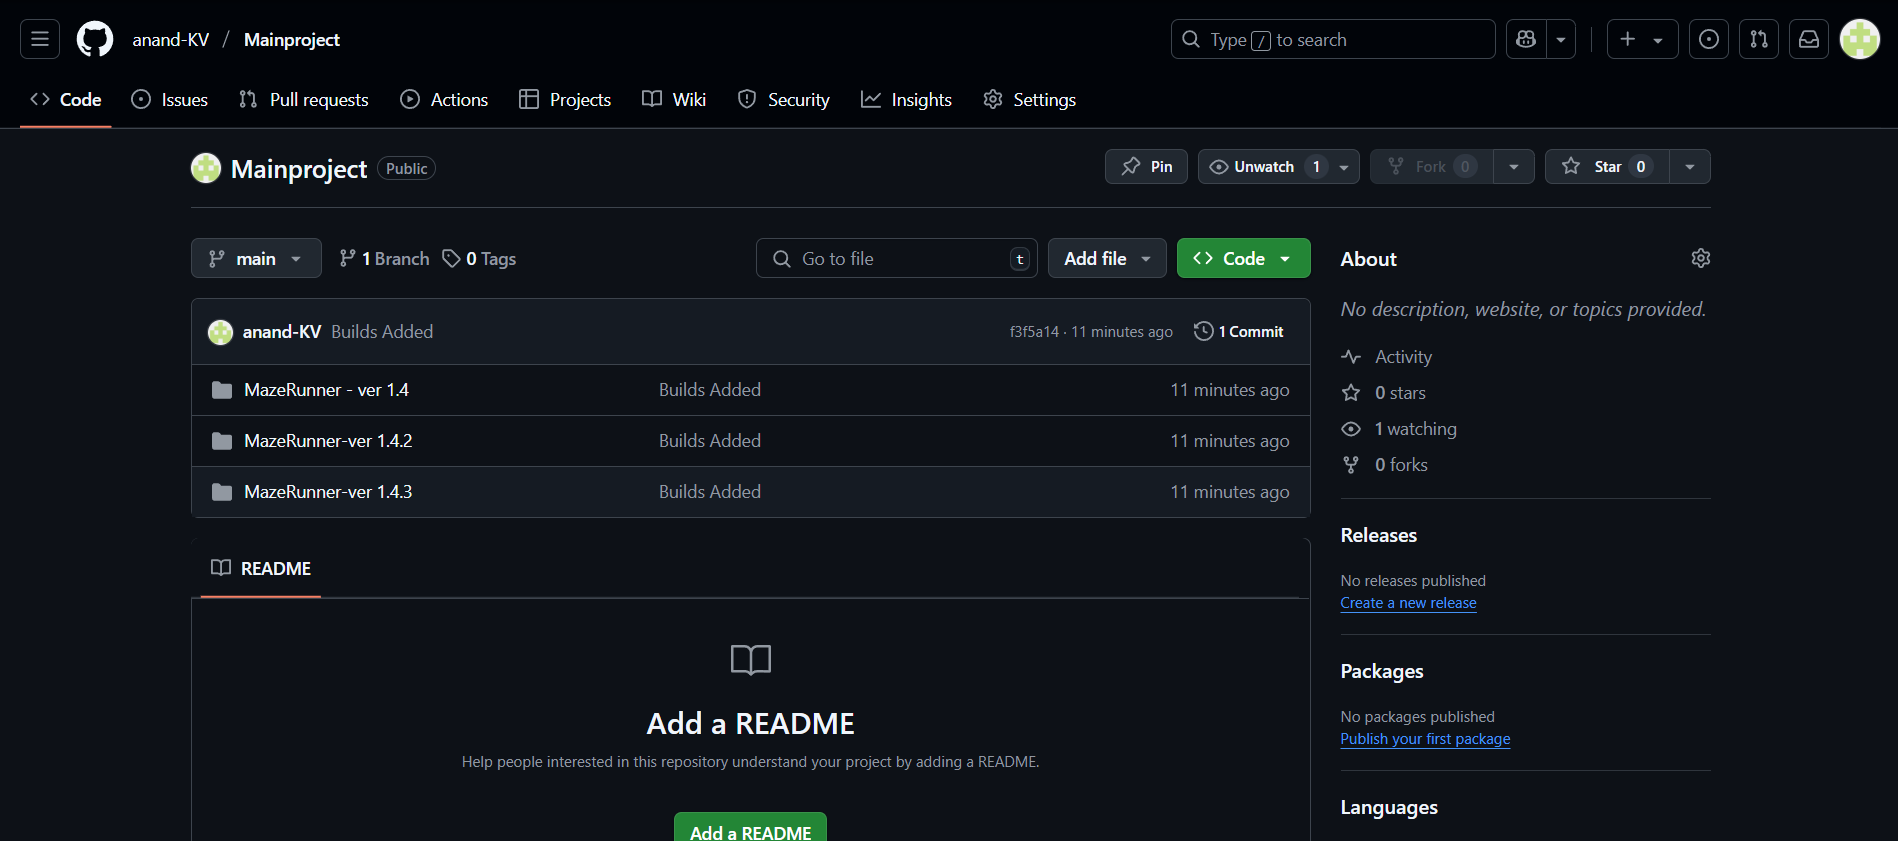
\includegraphics[width=1\textwidth]{git_1.png}
    \caption{Git Commit History -- AIRES Repository}
    \label{fig:git_history}
\end{figure}
\begin{figure}[H]
    \centering
    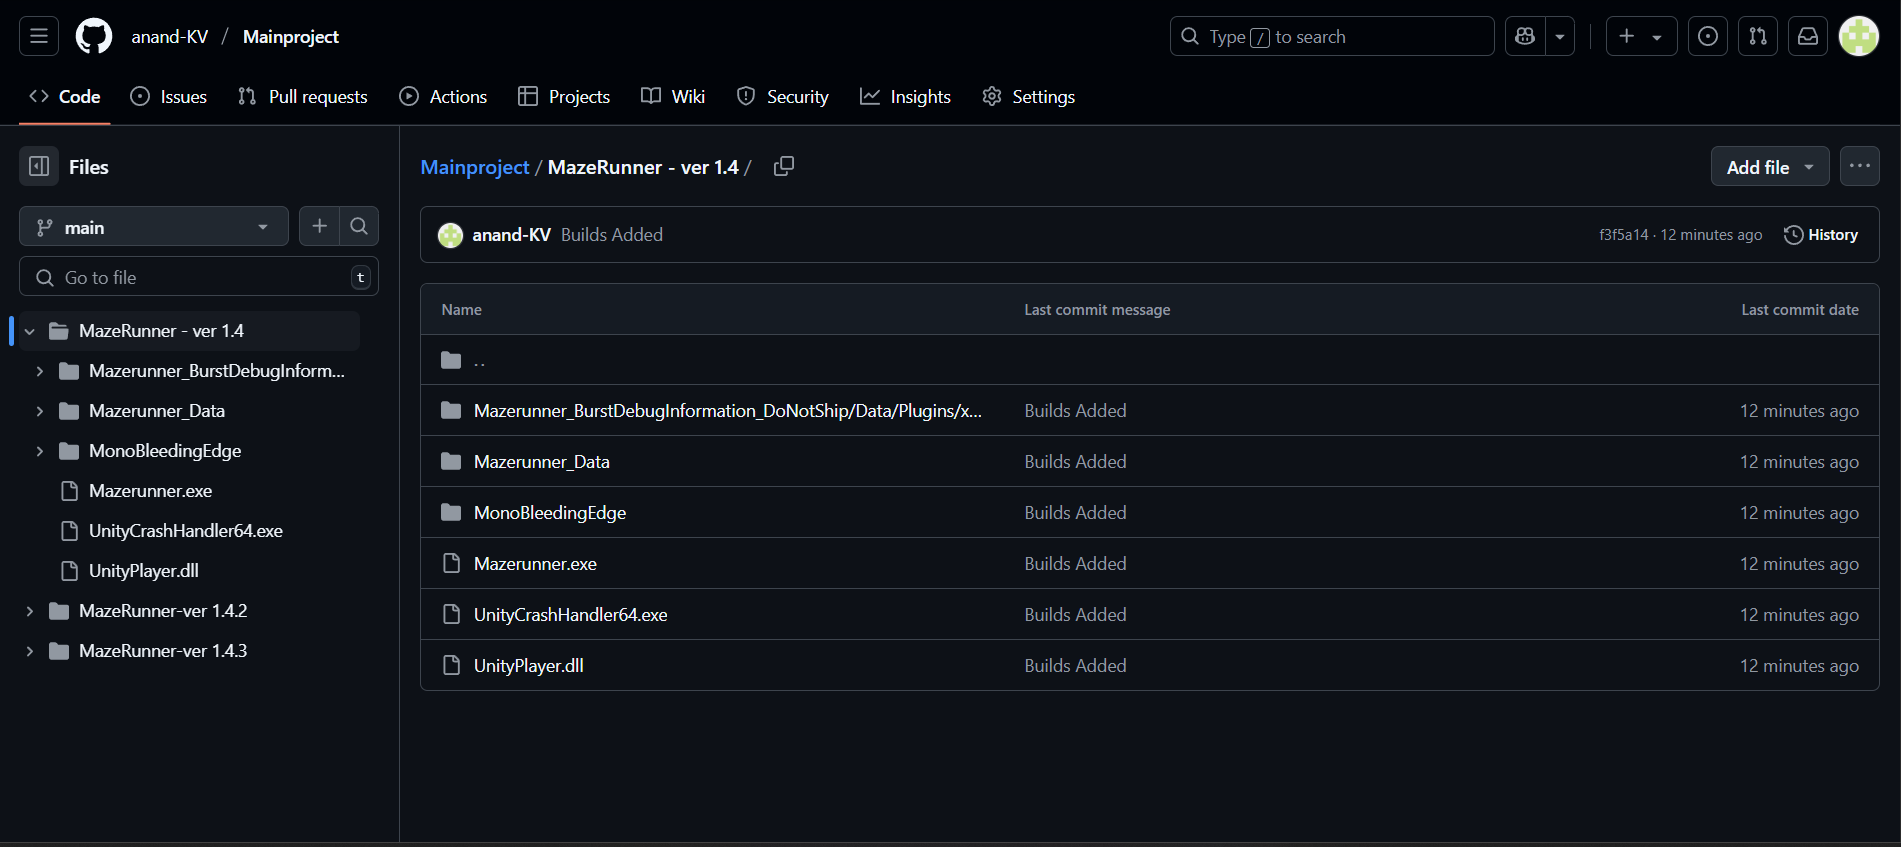
\includegraphics[width=1\textwidth]{build_in.png}
    \caption{Repository Files and Folder Structure on GitHub}
    \label{fig:git_files}
\end{figure}